\documentclass{article}
\usepackage[utf8]{inputenc}
\usepackage{graphicx}

\title{Informe: Actividad 1 "Enunciados". IS453-G1}
\author{Kevin Esguerra Cardona - 1004 699 587}
\date{\today}

\begin{document}
\maketitle

En el presente documento se consigna el informe de la actividad número 1 realizada en el curso de Programación 3 (Enunciados) en la cual se le pide al estudiante
realizar una serie de consultas simples al intérprete del lenguaje progol, previa base de datos suministrada, e interpretar tanto las peticiones enviadas cómo las 
respuestas recibidadas. 

\section*{Base de datos.}
Esta, es una base datos sencilla que contiene el arbol genealógica de una familia.
\begin{figure}[h]
    \centering
    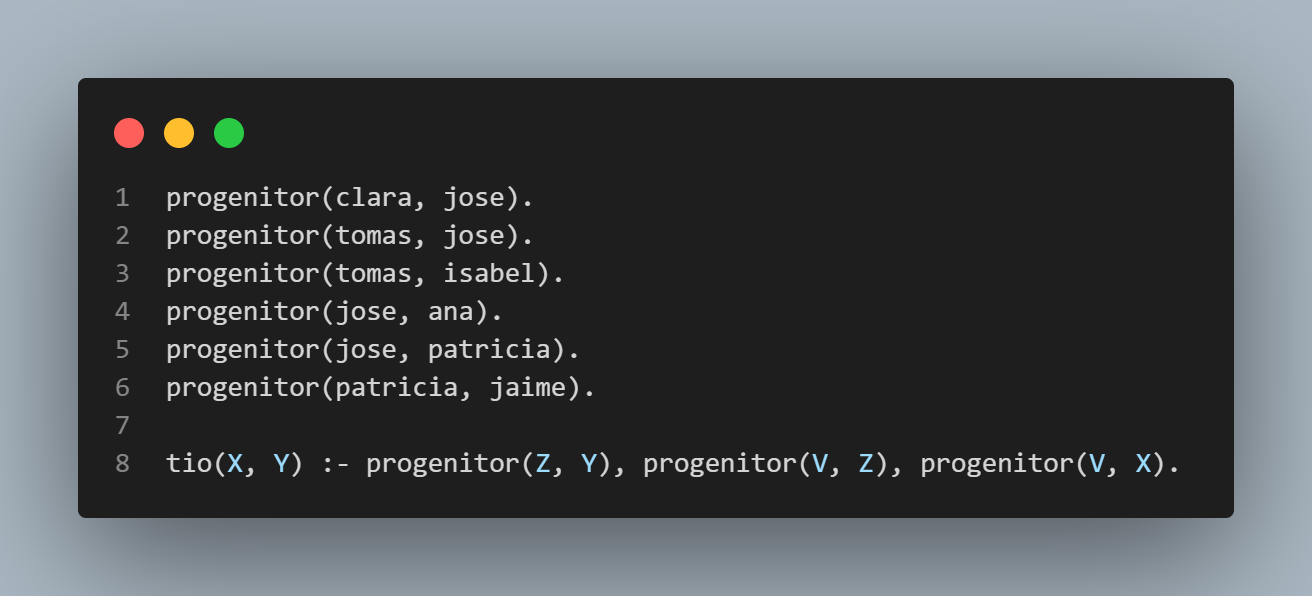
\includegraphics[width=1\textwidth]{./img/db.png}
    \caption{Base de datos utilizada en todos los ejercicios de la actividad.}
    \label{fig:db}
\end{figure}

\newpage
\section*{Ejercicio primero, resultados.}
En este ejercicio se pide la respuesta de prolog y el enunciado verbal a las siguientes consultas:
\begin{enumerate}
    \item ?-progenitor(jaime, X).
    \item ?-progenitor(X, jaime).
    \item ?-progenitor(clara, X), progenitor(X, patricia).
    \item ?-progenitor(tomas, X), progenitor(X, Y), progenitor(Y, Z).
\end{enumerate}

Peticiones, cuyas respuestas, en orden de llamada, fueron:
\begin{figure}[h]
    \centering
    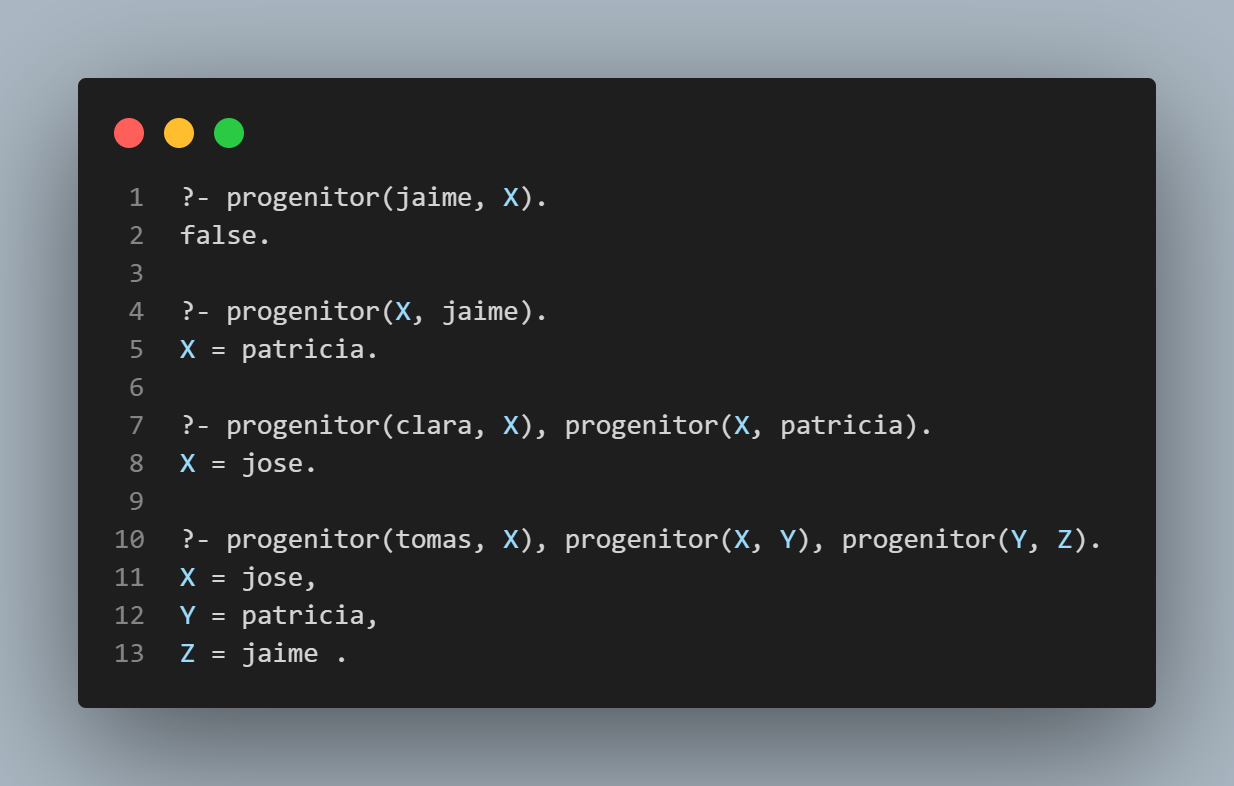
\includegraphics[width=1\textwidth]{./img/results.png}
    \caption{Resultados del primer ejercicio.}
    \label{fig:results_1}
\end{figure}

Y, en el mismo orden, sus posibles enunciados verbales serían:
\begin{enumerate}
    \item ¿Jaime es progenitor de quién? R: false. Es decir, Jaime no posee progenie.
    \item ¿Jaime es progenie de quién? R: Patricia. Es decir, Jaime es progenie de Patricia.
    \item ¿Quién progenitor de Patricia, que a su vez, es progenie de Clara? R: Jose. Es decir, Jose es progenie de Clara y progenitor de Patricia.
    \item ¿Quién progenie de la progenie de la progenie de Tomas? R: Jaime. Es decir, La progenie de Tomas, es progenitor del progenitor de Jaime. 
\end{enumerate}


\section*{Ejercicio segundo, resultados}
En este ejercicio se le pide al estudiante formular al interprete de prolog las siguientes preguntas, dadas en lenguaje natural:
\begin{enumerate}
    \item ¿Quién es el progenitor de Patricia?
    \item ¿Tiene Isabel un hijo o una hija?
    \item ¿Quién es el abuelo de Isabel?
    \item ¿Cuáles son los tíos de Patricia? (no excluir al padre)
\end{enumerate}

Preguntas, cuyas interpretaciones y resultados se ven a continuación: 
\begin{figure}[h]
    \centering
    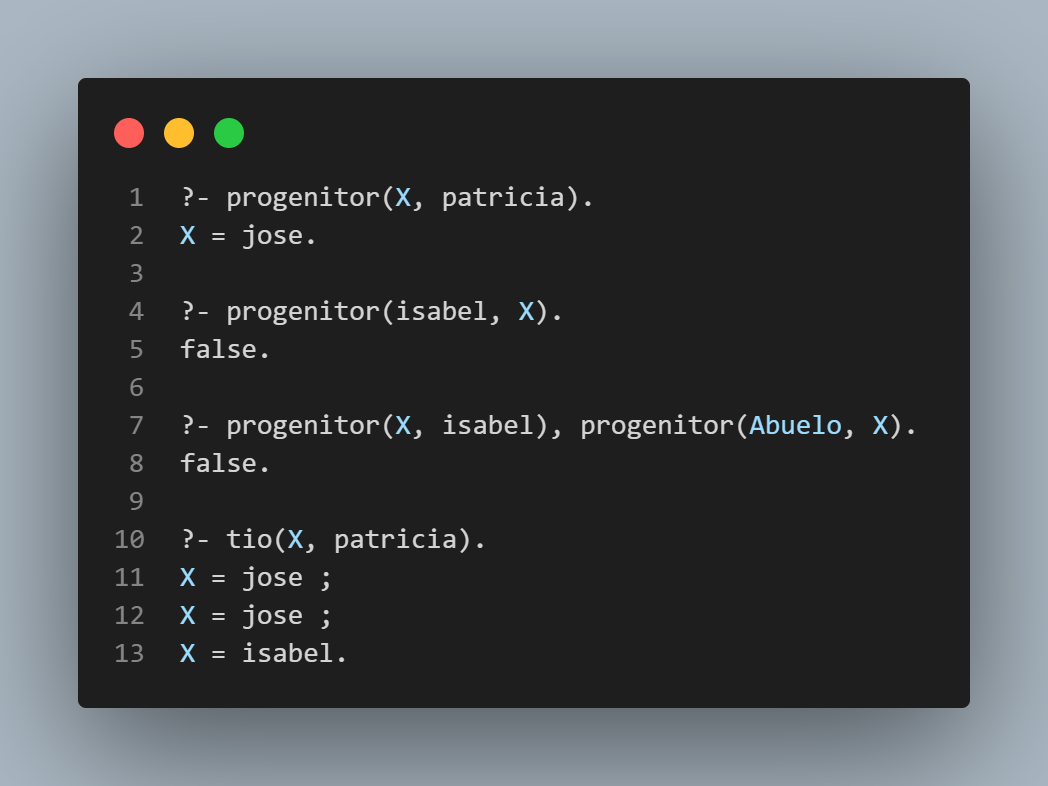
\includegraphics[width=1\textwidth]{./img/results_2.png}
    \caption{Resultados del segundo ejercicio.}
    \label{fig:results_2}
\end{figure}

Cabe a aclarar, que en el último caso jose aparece dos veces debido a la naturaleza no excluyente de la formulación realizada a prolog, pues esta busca los hijos de los abuelos de patricia, patricia tiene dos abuelos que son padres de jose, por esta razón jose aparece dos veces en los resultados.


\section*{Ejercicio tercero, resultados}
En este ejercicio se le pide al estudiante que, dadas 5 cláusulas nuevas previamente establecidas, escriba las reglas de Prolog que expresen las siguientes relaciones:

\begin{enumerate}
    \item es\_madre(X).
    \item es\_padre(X).
    \item es\_hijo(X).
    \item hermana\_de(X, Y).
    \item abuelo\_de(X, Y) y abuela\_de(X, Y).
    \item hermanos(X, Y).
    \item tia(X, Y). Excluid a los padres.
\end{enumerate}

Cuya interpretación resulta en:
\begin{figure}[h]
    \centering
    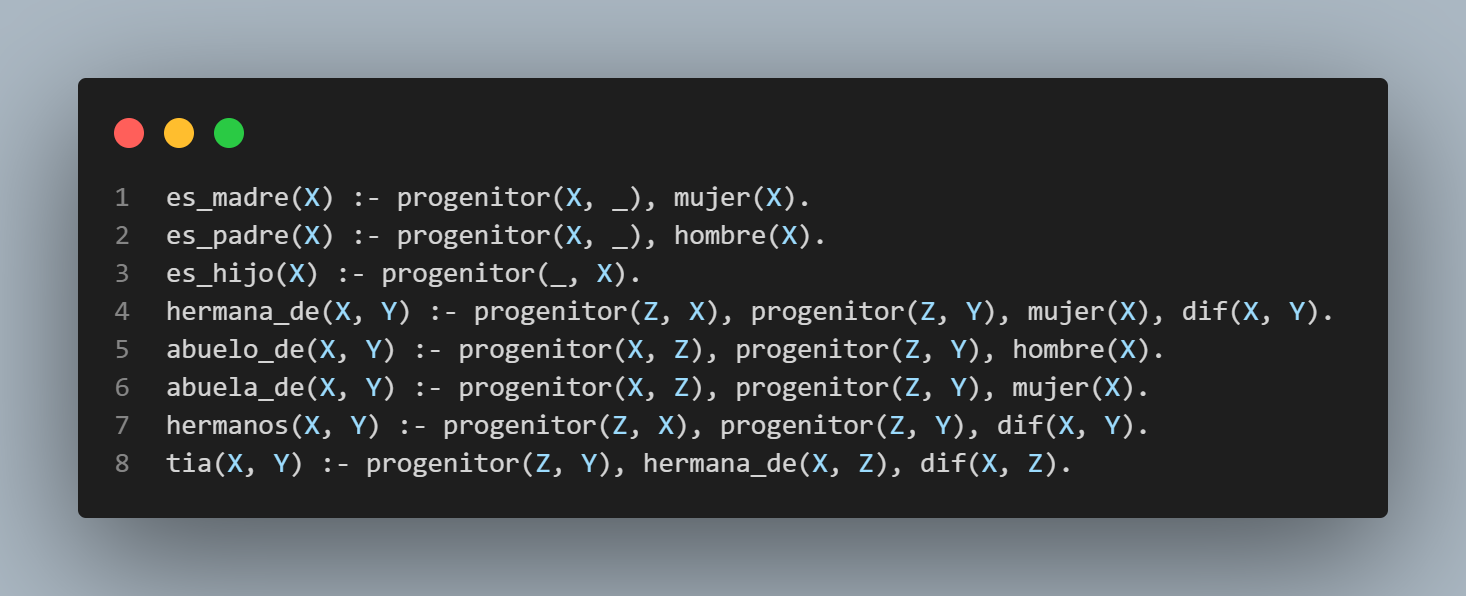
\includegraphics[width=1\textwidth]{./img/results_4.png}
    \caption{Interpretaciones del tercer ejercicio.}
    \label{fig:results_4}
\end{figure}

Y cuyas pruebas son, por ejemplo:
\begin{itemize}
    \item es\_madre(clara): false.
    \item es\_madre(jose): false.
    \item es\_madre(patricia): true.
    \item es\_padre(tomas): true.
    \item es\_padre(isabel): false.
    \item es\_hijo(jose): true.
    \item es\_hijo(clara): false.
    \item hermana\_de(isabel, patricia): true.
    \item hermana\_de(patricia, ana): false.
    \item abuelo\_de(tomas, ana): true.
    \item abuela\_de(clara, jaime): true.
    \item hermanos(jose, isabel): true.
    \item hermanos(patricia, jaime): false.
    \item tia(isabel, jaime): true.
    \item tia(tomas, ana): false.
  \end{itemize}  

\section*{Conclusión}
Al realizar esta actividad, he podido comprender, aunque en raza profundidad, la naturaleza de este lenguaje de programación y, más importante aún, de este paradigma. He utilizado conectores lógicos cómo el operador Y (,) y la implicación (:-). Entre otros. Estos me sirvieron para profundizar un poco más en la naturaleza de la lógica y de lo que debo esperar de esta primera parte del curso de programación 3.

\end{document}